% 将本书的 pic/ 目录下所有图片,按文件名顺序显示出来。
% 方便快速查找图片,以便借鉴其实现。
\documentclass[UTF8, 11pt, oneside]{ctexbook}
% 定义本书中使用到的格式

\ctexset {
  chapter = {
    pagestyle = headings,
  },
  section = {
     aftername={、},
  }
}

\usepackage{array}
\usepackage{mathtools} % 会自动加载宏包 'amsmath'
\allowdisplaybreaks[1]
\usepackage{amssymb}
\usepackage{bm}
\usepackage{calc}
\usepackage{caption}
\captionsetup[figure]{labelsep=none}
\usepackage{cases}

\usepackage{CJKfntef}
\usepackage{enumitem}
\usepackage{extarrows}
\usepackage{etoolbox}
\usepackage{float}
\usepackage[stable]{footmisc}
\usepackage{geometry}
\geometry{a4paper,left=2cm,right=2cm,top=2cm,bottom=1cm}

\usepackage{hyperref}
\hypersetup{colorlinks=true, linkcolor=red}

\usepackage{scalerel}

\usepackage{tabularray}
\UseTblrLibrary{counter}
\UseTblrLibrary{diagbox}
\UseTblrLibrary{siunitx}

\usepackage{tikz}
\usetikzlibrary{
  3d,
  angles,
  arrows.meta,
  calc,
  decorations.pathmorphing,
  decorations.pathreplacing,
  math,
  graphs,
  intersections,
  patterns,
  patterns.meta,
  positioning,
  quotes,
  shapes.geometric,
}
\usepackage{tikz-3dplot}

\usepackage{wrapfig}
\usepackage{xparse}
\usepackage{xpinyin}

\usepackage{tkz-euclide}
\tkzSetUpPoint[fill=black]
\tkzSetUpCompass[color=orange,line width=.3 pt]

% 《几何》中的公理、定理、推论,有的有编号,有的又没有。
%  而内容中,有的部分是黑体,又或间隔有(用于解释的)普通文本。
%  所以很难统一规则。
%  为了最大限度的复原原课本,故不采用 \newtheorem 定义的环境,
%     \newtheorem{theorem}{定理}[subsection]
%  而是自己定义一些简单的环境。
\NewDocumentEnvironment{xingzhi}{o}{% 性质
  \bfseries
  \IfNoValueF {#1}
    {#1 }%
}{}

\NewDocumentEnvironment{gongli}{o}{% 公理
  \bfseries
  \IfNoValueF {#1}
    {#1 }%
}{}
\NewDocumentEnvironment{dingli}{o}{% 定理
  \bfseries
  \IfNoValueF {#1}
    {#1 }%
}{}
\NewDocumentEnvironment{tuilun}{o}{% 推论
  \bfseries
  \IfNoValueF {#1}
    {#1 }%
}{}


% 确保 有行内公式 的行,与其上、下行之间,有足够的行距
% 参数1: 最后一行需要额外增加的高度(用于调整和后继行的间隔)
\NewDocumentEnvironment{enhancedline}{o}{
  \setlength{\lineskip}{\baselineskip-\ccwd}
  \setlength{\lineskiplimit}{2.5pt}
}{
  \IfValueT{#1}{
    \vspace{#1}
  }
  \par
}

% 绘制带圈的数字
\newcommand{\circled}[2][]{\tikz[baseline=(char.base)]
    {\node[shape = circle, draw, inner sep = 1pt]
    (char) {\phantom{\ifblank{#1}{#2}{#1}}};%
    \node at (char.center) {\makebox[0pt][c]{#2}};}}
\robustify{\circled}
\newcommand{\tc}[1]{\text{\circled{#1}}}

\counterwithout*{subsection}{section}
\counterwithin*{subsection}{chapter}
\setcounter{secnumdepth}{3}
\renewcommand{\thesection}{\chinese{section}}
\renewcommand{\thesubsection}{\arabic{chapter}.\arabic{subsection}}
\renewcommand{\thesubsubsection}{\arabic{subsubsection}.}

\renewcommand{\thefigure}{\thechapter-\arabic{figure}\;}
\renewcommand{\thetable}{\thechapter{}-\arabic{table}}
\renewcommand{\thefootnote}{\circled{\arabic{footnote}}}

% 在不改变 counter 值的情况下,重置 counter 的子 counter
\newcommand{\touchcounter}[1]{\stepcounter{#1} \addtocounter{#1}{-1}}

\newenvironment{starred}{
  \ctexset {
    chapter/name={*第,章},
    section/name={*},
    subsection/name={*},
  }
}{}


% 没有编号但又需要添加到目录中的 section (No num(ber) section)。
% 参数1: 目录中的文字(可选,如果没有指定,则使用参数2的值)
% 参数2: 正文中的文字
\NewDocumentCommand{\nonumsection}{o m}{%
  \touchcounter{section}
  \section*{#2}
  \IfNoValueTF{#1}
    {\addcontentsline{toc}{section}{#2}}
    {\addcontentsline{toc}{section}{#1}}
}

% 没有编号但又需要添加到目录中的 subsection (No num(ber) subsection)。
% 参数1: 目录中的文字(可选,如果没有指定,则使用参数2的值)
% 参数2: 正文中的文字
\NewDocumentCommand{\nonumsubsection}{o m}{%
  \touchcounter{subsection}
  \subsection*{#2}
  \IfNoValueTF{#1}
    {\addcontentsline{toc}{subsection}{#2}}
    {\addcontentsline{toc}{subsection}{#1}}
}


% (编号前)带星号的 subsection
% 参数1: subsection 的标题
% \NewDocumentCommand{\starredsubsection}{o m}{
%   \refstepcounter{subsection}
%   \subsection*{*\thesubsection\quad #2}
%   \IfNoValueTF{#1}
%     {\addcontentsline{toc}{subsection}{\makebox{*}\thesubsection\qquad #2}}
%     {\addcontentsline{toc}{subsection}{\makebox{*}\thesubsection\qquad #1}}
% }

\newcounter{cntliti}[subsection]           % 例题的计数器
\NewDocumentCommand{\liti}{o}{ % 例题的标题
  \IfNoValueTF{#1} {
    \stepcounter{cntliti}
    \textbf{例 \thecntliti}
  } {
    \textbf{例}
  }
  \;
}

\newcommand{\jie}{\textbf{解: }}
\newcommand{\zhengming}{\textbf{证明: }}

\newcounter{huafa}
\NewDocumentCommand{\huafa}{o} {
  \IfNoValueTF{#1}
    {\textbf{画法:}}
    {\setcounter{huafa}{#1} \textbf{画法\chinese{huafa}:}}
}
\newcommand*\zuofa{\textbf{作法:}}


\newenvironment{lianxi}{
  \vspace*{1em}
  {\large\textbf{练 \; 习}}\par
  \setcounter{cntxiaoti}{0}
  \begin{xiaotis}
}{
  \end{xiaotis}
  \vspace*{1em}
}

\newcounter{cntxiti}               % “习题”的计数器
\newcommand{\xiti}{%
  \stepcounter{cntxiti}
  \vspace{1em}
  {\centering \nonumsubsection{\labelxiti}}%在目录中显示“习题”
}
\newcommand{\labelxiti}{习题 \chinese{cntxiti}}


\newcommand{\xiaojie}{%
  \nonumsection[\labelxiaojie]{\Large \labelxiaojie}
}
\newcommand{\labelxiaojie}{小 \hspace{2em} 结}


\newcounter{cntfuxiti}                       % “复习参考题”的计数器
\newcommand{\fuxiti}{%
  \stepcounter{cntfuxiti}
  \nonumsection[\labelfuxiti]{\Large \labelfuxiti}
}
\newcommand{\labelfuxiti}{复习参考题\chinese{cntfuxiti}}

\newcounter{cntxiaoti}[subsubsection]      % 小题的计数器
\newcounter{cntxiaoxiaoti}[cntxiaoti]      % 小小题的计数器
\counterwithin*{cntxiaoti}{cntxiti}
\counterwithin*{cntxiaoti}{cntfuxiti}
\counterwithin*{cntxiaoxiaoti}{cntliti}
\newcommand{\resetxxt}{\setcounter{cntxiaoxiaoti}{0}} % 重置 小小题的计数器

\newlength{\lenLabel}                     % 内部变量:用于计算题目前编号所占的长度
\newlength{\lenParent}                    % 内部变量:用于记录父题目编号所占的长度
\setlength{\lenParent}{0em}

\newenvironment{xiaotis}{% “小题” 环境
  \NewDocumentCommand \xiaoti {s m} {% 小题的标题
    \IfBooleanTF {##1}%
      {%
        \setlength{\lenLabel}{\widthof{\labelxiaoti}}%
        \hangafter 1\setlength{\hangindent}{\parindent + \lenLabel}{\hspace{\lenLabel}##2}%
      }%
      {%
        \stepcounter{cntxiaoti}%
        \setlength{\lenLabel}{\widthof{\labelxiaoti}}%
        \hangafter 1\setlength{\hangindent}{\parindent + \lenLabel}{\labelxiaoti ##2}%
      }%
  }%
  \newcommand{\labelxiaoti}{\arabic{cntxiaoti}. }% 1. 2. 3. ……
  \newenvironment{withstar}{%
    \renewcommand{\labelxiaoti}{*\arabic{cntxiaoti}. }% 1. 2. 3. ……
  }{%
  }
}{%
}

% 为命令 `\xiaoxiaoti' 增加一个可选参数,是为了实现:当“小题”没有文字时,第一个“小小题” 与“小题”同行。
% 对应 《代数二》“习题 十四” 中的第 10 小题。
% 在此之前,是通过将 “小小题” 上移一行来实现同行显示。如:《代数二》“习题 七” 中的第 10 小题。
% 但当“小题”本身处于页的最后一行时,上移不能生效,会导致“小题”显示在上一页的页末,而“小小题”显示在下一页的页首。
\newenvironment{xiaoxiaotis}{% “小小题” 环境
  \setlength{\lenParent}{\lenParent + \lenLabel}%
  \NewDocumentCommand{\xiaoxiaoti}{o m} {% 小小题的标题
    \stepcounter{cntxiaoxiaoti}%
    \setlength{\lenLabel}{\widthof{\labelxiaoxiaoti}}%
    \IfNoValueTF{##1}%
      {\hangafter 1\setlength{\hangindent}{\parindent + \lenParent + \lenLabel + 0.5em}{\hspace{\lenParent}~\labelxiaoxiaoti ##2}}%
      {\hangafter 1\setlength{\hangindent}{\parindent + \lenParent + \lenLabel + 0.5em}{\hspace{##1}~\labelxiaoxiaoti ##2}}%
  }%
  \newcommand{\labelxiaoxiaoti}{(\arabic{cntxiaoxiaoti})}% (1) (2) (3) ……
  % 小小题 与 小题 同行时的默认缩进。调用形式为: \xiaoxiaoti[\xxtsep]{小小题的内容}
  \newcommand{\xxtsep}{0em}%
  \def\xxt{\xiaoxiaoti}%定义一个缩写。因为在表格中,如果总写 \xiaoxiaoti,字数太多。影响阅读。
}{%
}

\newcommand{\ewkh}[1][2em]{(\hspace{#1})}%英文括号
\newcommand{\xhx}[1][2em]{\CJKunderline{\hspace{#1}}}%下划线

\newcommand{\twoInLine}  [3][10em] {\begin{tabular}[t]{*{2}{@{}p{#1}}} #2 & #3\end{tabular}}
\newcommand{\threeInLine}[4][10em] {\begin{tabular}[t]{*{3}{@{}p{#1}}} #2 & #3 & #4\end{tabular}}
\newcommand{\fourInLine} [5][10em] {\begin{tabular}[t]{*{4}{@{}p{#1}}} #2 & #3 & #4 & #5\end{tabular}}

\newcommand{\twoInLineXxt}  [3][10em] {\begin{tabular}[t]{*{2}{@{}p{#1}}} \xiaoxiaoti{#2} & \xiaoxiaoti{#3}\end{tabular}}
\newcommand{\threeInLineXxt}[4][10em] {\begin{tabular}[t]{*{3}{@{}p{#1}}} \xiaoxiaoti{#2} & \xiaoxiaoti{#3} & \xiaoxiaoti{#4}\end{tabular}}
\newcommand{\fourInLineXxt} [5][10em] {\begin{tabular}[t]{*{4}{@{}p{#1}}} \xiaoxiaoti{#2} & \xiaoxiaoti{#3} & \xiaoxiaoti{#4} & \xiaoxiaoti{#5}\end{tabular}}

\newcommand{\shangyihang}{\vspace{-1.2em}} % 上移一行
\newcommand{\jiange}{\vspace{0.5em}} % 手工调整垂直间隔(测试发现 0.5em 比较合适。不支持参数,特殊情况直接使用 \vspace{} 命令。)
\newcommand{\lianxijiange}{\vspace{2em}} % “练习” 与后继内容之间的间隔
\newcommand{\huitui}{\hspace*{-1em}} % 回退。

% 修改数学公式与上下文的距离
\makeatletter
\renewcommand\normalsize{%
    \abovedisplayskip 1\p@ \@plus1\p@ \@minus6\p@
    \belowdisplayskip \abovedisplayskip
}
\makeatother

\newcommand{\exdfrac}[2]{\dfrac{\; #1 \;}{#2}}% \dfrac{a}{b}这样只有一个字符的式子,分数线太短。本命令通过 \; 来增加分数线的长度。

%----------------------------------
\counterwithin*{equation}{subsection}
\renewcommand{\theequation}{\arabic{equation}}

\makeatletter
% 创建指定名字的标签
% 参数1: 标签的id
% 参数2: 标签的名字 (\nameref{标签id} 所得到的结果)
\newcommand{\namedlabel}[2]{%
  \@bsphack%
  \protected@write\@auxout{}{%
    \string\newlabel{#1}{%
        {\@currentlabel}%
        {\thepage}%
        {{#2}}%\@currentlabelname
        {\@currentHref}{}%
      }%
  }%
  \@bsphack%
}%
\makeatother

%----------------------------------
\newcounter{mylabel}
% 针对计数器 mylabel 创建(指定名字)标签
% 参数1: 标签的id
% 参数2: (可选) 标签的名字 (\nameref{标签id} 所得到的结果)。默认为标签归属章节的名字
\NewDocumentCommand{\mylabel}{m o}{%
  \refstepcounter{mylabel}%
  \IfValueTF{#2}{%
    \namedlabel{#1}{#2}%
  }{%
    \label{#1}%
  }%
}


%----------------------------------
% 实现类似如下效果:
%  name1 .............. value1
%  another-name2 .......... v2
\makeatletter
\newcommand \cdotfill {\leavevmode \cleaders \hb@xt@ .33em{\hss $\cdot$ \hss }\hfill \kern \z@}
\makeatother

\newenvironment{dottedlist}[2]{%
    \newcommand{\pair}[2]{\item ##1 \cdotfill ##2}
    \begin{itemize}[nosep, leftmargin=#1, rightmargin=#2]
        \renewcommand{\labelitemi}{}
}{%
    \end{itemize}
}


%---------------------------
\newcommand{\zhuyi}{\textbf{注意} \hspace{1em}}
\newcommand{\zhongdian}[1]{\textbf{#1}} % 重点(内容)

\newcommand{\shushi}[3]{% 竖式。
    % 注意,不要在 tblr 中调用此命令。只能在 tabular 中使用。
    \renewcommand\arraystretch{0.8}
    $\begin{array}[t]{r@{\;}r@{\quad}r}
        && #1 \\[-0.3em]
        #2 &  \vstretch{1.1}{\big)}\mkern-7.3mu & #3 \\
        \cline{2-3}
    \end{array}$
}

% 分隔
% 主要用于实现将 ∵ (或 ∴)符号 与 居中的数学公式显示在同一行。
% 参数1: (可选) 右侧的宽度。缺省为 0.9\textwidth
% 参数2: 左侧要显示的内容。一般为 $\because$ 或 $\therefore$
% 参数3: 右侧要显示的(居中的)数学公式。
% 示例:
% \fenge{$\because$}{$$ \text{左边} \neq \text{右边} $$}
% \fenge{$\therefore$}{\begin{equation} a=b \end{equation}}
\newcommand{\fenge}[3][0.9\textwidth]{
  #2 \begin{minipage}{#1}
    #3
  \end{minipage}
}
\newcommand{\fengeYinwei}[1]{\fenge{$\because$}{$$#1$$}}
\newcommand{\fengeSuoyi}[1]{\fenge{$\therefore$}{$$#1$$}}


%------------------------
\NewTblrTheme{nocaption}{
  \DefTblrTemplate{caption}{default}{}
  \DefTblrTemplate{caption-tag}{default}{}
  \DefTblrTemplate{caption-sep}{default}{}
  \DefTblrTemplate{contfoot-text}{default}{未完待续}
  \DefTblrTemplate{conthead-text}{default}{(续表)}
}


\NewTblrEnviron{datatblr}
\SetTblrInner[datatblr]{rows={mode=math, r, rowsep=0pt}}
\newenvironment{data}{
  \vspace*{-0.5em}\begin{center}
}{
  \end{center}\vspace*{-0.5em}
}

\NewTblrEnviron{statisticstblr}
\SetTblrInner[statisticstblr]{hlines, vlines, rows={mode=math, c}, row{1}={mode=text}, column{2}={mode=text, l}, columns={colsep=1em}}

\NewTblrEnviron{zmtblr}% 证明用的 tblr
\SetTblrInner[zmtblr]{colsep=0pt, rowsep=0pt}

%----------------------------------
% (重)定义一些数学符号
%  一是为了使用/记忆上的方便,二是如果以后有变动,只需要修改一处。
\newcommand{\celsius}{\ensuremath{^\circ\hspace{-0.09em}\mathrm{C}}} % 摄氏度
\newcommand*\xiangsi{%                 % 相似 (如果不在意有些不同,可以使用 \backsim )
    \mathrel{\text{%
            \tikz \draw[baseline] (-.25em,1.15ex) .. controls (-.55em,1.15ex) and (-.51em,.23ex) .. (-.275em,.23ex) .. controls (0,.23ex) and (0,1.15ex) .. (.275em,1.15ex) .. controls (.51em,1.15ex) and (.55em,.23ex) .. (.25em,.23ex);%
}}}
\newcommand\pingxing{% 平行
    \mathrel{\tikz[baseline] \draw (0em,-0.3ex) -- (.4em,1.7ex) (.2em,-0.3ex) -- (.6em,1.7ex);%
}}
\newcommand*\quandeng{% 全等
  \mathrel{%
    \tikz \draw[baseline] (-.2em,1.35ex) .. controls (-.46em,1.6ex) and (-.54em,.65ex) .. (-.25em,.65ex) .. controls (-.06em,.65ex) and (.06em,1.35ex) .. (.25em,1.35ex) .. controls (.54em,1.35ex) and (.46em,.4ex) .. (.2em,.65ex) (-.46em,.4ex) -- (.46em,.4ex) (-.46em,0ex) -- (.46em,0ex);%
}}
%平行四边形
\newcommand*\Pxsbx[1][1]{%
    \mathord{%
        \tikz[baseline,scale=#1]
        \draw (0,.1ex) -- (.8em,.1ex) -- (1em,1.4ex) -- (.2em,1.4ex) -- cycle;}}
\newcommand*\pxsbx{
    \mathchoice{\Pxsbx}{\Pxsbx}{\Pxsbx[0.6]}{\Pxsbx[0.4]}
}
%平行且等于
\newcommand*\pxqdy{%
    \mathrel{\tikz[baseline]
        \draw (.1em,.25ex) -- (.9em,.25ex)
        (.1em,-.25ex) -- (.9em,-.25ex)
        (.305em,.25ex) -- (.605em,1.5ex)
        (.525em,.25ex) -- (.825em,1.5ex);%
}}

%特殊符号
\newcommand{\nsep}{,\quad}% 连续的数字之间的分隔符
\newcommand{\douhao}{\mathord{\text{,}}}%(中文的)逗号
\newcommand{\juhao}{\mathord{\text{。}}}%(中文的)句号
\newcommand{\fenhao}{\mathord{\text{;}}}%(中文的)分号
\newcommand{\dao}{\mathord{\text{~}}}%(中文的)波浪号

% “正” 字的五步
\newcommand{\za}{\hbox{\lower-0.8ex\hbox{\scalebox{0.9}[1]{一}}}}
\newcommand{\zb}{丅}
\newcommand{\zc}{\hbox{丅{\kern-.5em\lower0.1ex\hbox{\scalebox{0.4}[1]{一}}}}}
\newcommand{\zd}{\hbox{丅{\kern-.5em\lower0.1ex\hbox{\scalebox{0.4}[1]{一}}}{\kern-1.2em\lower0.1ex\hbox{\scalebox{1}[0.6]{丨}}}}}
\newcommand{\ze}{正}


%方程
\newcommand{\zuobian}{\text{左边}}
\newcommand{\youbian}{\text{右边}}

%------------------ 物理单位
% 长度单位
\newcommand{\qianmi}{\mathord{\text{km}}}%千米
\newcommand{\mi}{\mathord{\text{m}}}%米
\newcommand{\fenmi}{\mathord{\text{dm}}}%分米
\newcommand{\limi}{\mathord{\text{cm}}}%厘米
\newcommand{\haomi}{\mathord{\text{mm}}}%毫米
\newcommand{\weimi}{\mathord{\text{um}}}%微米

% 面积单位
\newcommand{\pfqm}{\mathord{\text{千米}^2}}%平方千米
\newcommand{\pfm}{\mathord{\text{m}^2}}%平方米
\newcommand{\pflm}{\mathord{\text{cm}^2}}%平方厘米
\newcommand{\pfhm}{\mathord{\text{毫米}^2}}%平方毫米

% 体积单位
\newcommand{\lfm}{\mathord{\text{米}^3}}%立方米
\newcommand{\lffm}{\mathord{\text{分米}^3}}%立方分米
\newcommand{\lflm}{\mathord{\text{厘米}^3}}%立方厘米
\newcommand{\lfhm}{\mathord{\text{毫米}^3}}%立方毫米

% 质量单位
\newcommand{\haoke}{\mathord{\text{毫克}}}%毫克
\newcommand{\ke}{\mathord{\text{克}}}%克
\newcommand{\qianke}{\mathord{\text{千克}}}%千克

\newcommand{\qkmlfm}{\mathord{\text{千克}/\text{米}^3}}%千克每立方米
\newcommand{\kmlflm}{\mathord{\text{克}/\text{厘米}^3}}%克每立方厘米

% 力的单位
\newcommand{\niudun}{\mathord{\text{牛顿}}}%牛顿
\newcommand{\ndmqk}{\mathord{\text{牛顿/千克}}}%牛顿每千克
\newcommand{\ndmpfm}{\mathord{\text{牛顿}/\text{米}^2}}%牛顿每平方米
\newcommand{\pasika}{\mathord{\text{帕斯卡}}}%帕斯卡

% 功的单位
\newcommand{\niudunmi}{\mathord{\text{牛顿·米}}}%牛顿·米
\newcommand{\jiaoer}{\mathord{\text{焦耳}}}%焦耳
\newcommand{\jemm}{\mathord{\text{焦耳/秒}}}%焦耳每秒
\newcommand{\wate}{\mathord{\text{瓦特}}}%瓦特
\newcommand{\qianwa}{\mathord{\text{千瓦}}}%千瓦
\newcommand{\mali}{\mathord{\text{马力}}}%马力

% 时间单位
\newcommand{\miao}{\mathord{\text{秒}}}%秒
\newcommand{\xiaoshi}{\mathord{\text{小时}}}%小时

% 速度单位
\newcommand{\qmmm}{\mathord{\text{千米/秒}}}%千米/秒
\newcommand{\mmm}{\mathord{\text{米/秒}}}%米/秒
\newcommand{\lmmm}{\mathord{\text{厘米/秒}}}%厘米/秒
\newcommand{\mmf}{\mathord{\text{米/分}}}%米/分

% 热量单位
\newcommand{\qianka}{\mathord{\text{千卡}}}%千卡
\newcommand{\ka}{\mathord{\text{卡}}}%卡
\newcommand{\kmkssd}{\mathord{\text{卡/(克·℃)}}}%卡每克摄氏度
\newcommand{\qkmqkssd}{\mathord{\text{千卡/(千克·℃)}}}%千卡每千克摄氏度

% 电的单位
\newcommand{\kulun}{\mathord{\text{库仑}}}%库仑
\newcommand{\anpei}{\mathord{\text{安培}}}%安培
\newcommand{\fute}{\mathord{\text{伏特}}}%伏特
\newcommand{\oumu}{\mathord{\text{欧姆}}}%欧姆
\newcommand{\qianwashi}{\mathord{\text{千瓦时}}}%千瓦时
\newcommand{\du}{\mathord{\text{度}}}%度

%----------------------------------
% 图形相关的项
% 需要 TexLive 2020 版本

% 自定义填充格式,用于实现绘制阴影
% TikZ 提供的 north east lines 等默认 pattern, 或 Lines ,有个问题:使用不同的PDF阅读器,会得到不同的效果。
% 如:
%       VSCode 中 LaTeX WorkShop 看到的是线段,
%       SumatraPDF 看到的是连贯的线条。
% 所以这里采用自定义的格式。
% 下面的代码基本是将 Lines 的代码修改而成。
% Lines实现中,bounding box 是 (-0.5\distance, -0.5\distance) 到 (0.5\distance, 0.5\distance)
% 这里的 TikZ 实现是 (0, 0) 到 (\distance, \distance),按说应该没有区别,但实际效果确有不同。
\pgfdeclarepattern{
  name=mylines,
  parameters={
      \pgfkeysvalueof{/pgf/pattern keys/distance},
      \pgfkeysvalueof{/pgf/pattern keys/angle},
      \pgfkeysvalueof{/pgf/pattern keys/xshift},
      \pgfkeysvalueof{/pgf/pattern keys/yshift},
      \pgfkeysvalueof{/pgf/pattern keys/line width},
  },
  bottom left={%
    \pgfpoint
      {0}%
      {0}},
  top right={%
    \pgfpoint
      {(\pgfkeysvalueof{/pgf/pattern keys/distance})}%
      {(\pgfkeysvalueof{/pgf/pattern keys/distance})}},
  tile size={%
    \pgfpoint
      {\pgfkeysvalueof{/pgf/pattern keys/distance}}%
      {\pgfkeysvalueof{/pgf/pattern keys/distance}}},
  tile transformation={%
    \pgftransformshift{%
      \pgfpoint
        {\pgfkeysvalueof{/pgf/pattern keys/xshift}}%
        {\pgfkeysvalueof{/pgf/pattern keys/yshift}}}%
    \pgftransformrotate{\pgfkeysvalueof{/pgf/pattern keys/angle}}},
  defaults={
    distance/.initial=3pt,
    angle/.initial=0,
    xshift/.initial=0pt,
    yshift/.initial=0pt,
    line width/.initial=\the\pgflinewidth,
  },
  code={%
    \pgfsetlinewidth{\pgfkeysvalueof{/pgf/pattern keys/line width}}%
    \pgfpathmoveto{\pgfpoint{0pt}{0pt}}%
    \pgfpathlineto{\pgfpoint{(\pgfkeysvalueof{/pgf/pattern keys/distance})}{0pt}}%
    \pgfusepath{stroke}%
  },
}


% 绘制温度计(温度范围:-10 ~ 20 ℃)
\tikzset{
    % 参数1: 显示的温度。
    pics/thermometer/.style n args={1}{
      code = {
        % 绘制外框
        \draw [thick] (-1, -0.6) -- (0.8, -0.6) -- (0.8, 6) -- (-1, 6) -- cycle;

        % 绘制玻璃管
        \draw [thick] (135:0.35) arc (135:405:0.35)
            to [out=135, in=270] (0.2, 0.5)
            -- (0.2, 6) -- (-0.2, 6) -- (-0.2, 0.5)
            to [out=270, in=45] (135:0.35);

        % 绘制刻度
        \foreach \y in {1,...,7} {
            \ifnum \y<3
                \def\value{\the\numexpr5*(3-\y)}
            \else
                \def\value{\the\numexpr5*(\y-3)}
            \fi
            \draw (-0.2,0.5+0.7*\y) -- (-0.4,0.5+0.7*\y) node[anchor=east] {$\value$};
            \ifnum \y < 7
                \foreach \tmp in {1,...,4} {
                    \draw (-0.2,0.5+0.7*\y+0.14*\tmp) -- (-0.3,0.5+0.7*\y+0.14*\tmp);
                }
            \fi
        }

        % 绘制水银柱
        \def\h{\the\numexpr0.5+2.1+0.14*#1}
        \draw [black!80, fill] (135:0.3) arc (135:405:0.3)
            to [out=135, in=270] (0.15, 0.4)
            -- (0.15, \h) -- (-0.15, \h) -- (-0.15, 0.4)
            to [out=270, in=45] (135:0.3);
      }
    }
}


% 用于填充的水面的纹路
\tikzset{
    waterwave/.pic={
        \draw [dash=on 17pt off 2pt phase 0pt] (0, -0.01) -- (10, -0.01);
        \draw [dash=on 15pt off 3pt phase 0pt] (0, -0.1)  -- (10, -0.1);
        \draw [dash=on 10pt off 4pt phase 0pt] (0, -0.2)  -- (10, -0.2);
        \draw [dash=on 9pt off 3pt phase 0pt]  (0, -0.3)  -- (10, -0.3);
        \draw [dash=on 6pt off 2pt phase 0pt]  (0, -0.4)  -- (10, -0.4);
        \draw [dash=on 4pt off 2pt phase 0pt]  (0, -0.5)  -- (10, -0.5);
        \draw [dash=on 3pt off 2pt phase 0pt]  (0, -0.6)  -- (10, -0.6);
    }
}

% 路面样式(用于修改 Path)
\tikzset{
    ground/.style={ground/.cd, #1, wrapper},
    ground/.cd,
      angle/.initial=-45,
      wrapper/.style={/tikz/.cd,
        postaction={
          draw,
          decorate,
          decoration={
            border,
            angle=\pgfkeysvalueof{/tikz/ground/angle},
            amplitude=0.3cm,
            segment length=2mm}}
      },
}


% 绘制一个箭头。
% 共有四个参数:
%   1. (箭头下部矩形)的底的长度
%   2. (箭头下部矩形)的高的长度
%   3. (箭头上部三角形)的底的长度
%   4. (箭头上部三角形)的高的长度
% 调用的例子:
%   \draw [fill=white] (0, 0) pic {arrow={.2}{.3}{.4}{.2}};
%   \draw [red, thick, pattern=dots] (0, 0) pic [rotate=90] {arrow={.2}{.3}{.4}{.2}};
\tikzset{
    pics/arrow/.style n args={4}{
      code = {
        \filldraw [pic actions] (-#1/2, 0) -- (#1/2, 0) -- (#1/2, #2)
            -- (#3/2, #2) -- (0, #2+#4)
            -- (-#3/2, #2) -- (-#1/2, #2)
            -- cycle;
    }}}


% 绘制立方体 ( 代码改编自 https://tex.stackexchange.com/a/48776/121799 )
% 依赖的库:
%   \usetikzlibrary{3d}
% 共有六个参数:
%   1. X 的最小值
%   2. X 的最大值
%   3. Y 的最小值
%   4. Y 的最大值
%   5. Y 的最小值
%   6. Y 的最大值
% 调用举例:以步进 0.5,使用粗线条,绘制一个 3 * 2 * 2 的立方体。
%   \draw [step=0.5, thick] (0, 0) pic {cubes={0}{3}{0}{2}{0}{2}};
\tikzset{
    pics/cubes/.style n args={6}{
      code = {
        \def\XGridMin{#1}
        \def\XGridMax{#2}
        \def\YGridMin{#3}
        \def\YGridMax{#4}
        \def\ZGridMin{#5}
        \def\ZGridMax{#6}
         %
        \begin{scope}[canvas is xy plane at z=\ZGridMax]
            \draw [pic actions] (\XGridMin,\YGridMin) grid (\XGridMax,\YGridMax);
        \end{scope}
        \begin{scope}[canvas is yz plane at x=\XGridMax]
            \draw [pic actions] (\YGridMin,\ZGridMin) grid (\YGridMax,\ZGridMax);
        \end{scope}
        \begin{scope}[canvas is xz plane at y=\YGridMax]
            \draw [pic actions] (\XGridMin,\ZGridMin) grid (\XGridMax,\ZGridMax);
        \end{scope}
    }
  }
}


% 绘制两端有竖线的线段
\tikzset{
  xianduan/.style={xianduan/.cd, #1, wrapper},
  xianduan/.cd,
    above/.store in=\above,  above=0.5em,
    below/.store in=\below,  below=0.5em,
    wrapper/.style={/tikz/.cd, to path={
        ($(\tikztostart)!\above!90:(\tikztotarget)$)  -- ($(\tikztostart)!\below!-90:(\tikztotarget)$)
        ($(\tikztotarget)!\above!-90:(\tikztostart)$) -- ($(\tikztotarget)!\below!90:(\tikztostart)$)
        (\tikztostart) -- (\tikztotarget) \tikztonodes
    }}
}


% 绘制垂足
% 注:可以使用 Angle Library 提供的 right angle 替换掉本命令(chuizu)
\tikzset{
    chuizu/.style={chuizu/.cd, #1, wrapper},
    chuizu/.cd,
        size/.store in=\size,   size=0.5em,
        % (从上至下画线时)垂足在显示的方位:right表示显示在右侧(缺省值),left表示在左侧)
        direction/.is choice,
            direction/right/.code = {\def\chuizuangle{-90}},
            direction/left/.code  = {\def\chuizuangle{90}},
            direction=right,
        skipline/.is choice,
            skipline/true/.code  = {\def\mainpath{(\tikztostart)    (\tikztotarget)}},
            skipline/false/.code = {\def\mainpath{(\tikztostart) -- (\tikztotarget)}},
            skipline=false,
        wrapper/.style={/tikz/.cd, to path={
            ($(\tikztotarget)!\size!0:(\tikztostart)$)
                -- ($(\tikztotarget)!1.414*\size!0.5*\chuizuangle:(\tikztostart)$)
                -- ($(\tikztotarget)!\size!\chuizuangle:(\tikztostart)$)
            \mainpath \tikztonodes
        }}
}


% 在数轴上绘制区间
\tikzset{
  interval/.pic={
    \begin{scope}[interval options/.cd,#1]
      \pgfkeysgetvalue{/tikz/interval options/start}{\start}
      \pgfkeysgetvalue{/tikz/interval options/stop}{\stop}
      \pgfkeysgetvalue{/tikz/interval options/height}{\height}
      \pgfmathsetmacro{\sign}{\start < \stop ? 1 : -1}
      \pgfmathsetmacro{\posOne}{\sign * 0.2}
      \pgfmathsetmacro{\posTwo}{\sign * 0.5}

      \ifthenelse {\infinity = 1} {
        \draw (\start, 0) .. controls (\start+\posOne, \height) and (\start+\posTwo, \height) .. (\start+\posTwo, \height)
          -- (\stop, \height);
      } {
        \draw (\start, 0) .. controls (\start+\posOne, \height) and (\start+\posTwo, \height) .. (\start+\posTwo, \height)
          -- (\stop-\posTwo, \height) .. controls (\stop-\posTwo, \height) and (\stop-\posOne, \height) .. (\stop, 0);
      }
    \end{scope}
  },
  interval options/.is family,
  interval options/.cd,
    start/.initial=0,    % 指定参数 start 的默认值
    stop/.initial=1,     % 指定参数 stop 的默认值
    height/.initial=1,   % 指定参数 height 的默认值
    infinity/.is choice, % 是否是 无限区间。 true: 无限区间; false: 有限区间。
      infinity/true/.code  = {\pgfmathsetmacro{\infinity}{1}},
      infinity/false/.code = {\pgfmathsetmacro{\infinity}{0}},
      infinity=false,    % 缺省为:有限区间
}


% 绘制 “十字相乘法”
% 共有四个参数:
%   1. a_1
%   2. a_2
%   3. c_1
%   4. c_2
\tikzset{
  pics/cross/.style n args={4}{
    code = {
      \begin{scope}[every node/.style={minimum width=3em}]
        \node [align=right] (a1) at (0, 1) {$#1$};
        \node [align=right] (a2) at (0, 0) {$#2$};
        \node [align=left] (c1) at (3, 1) {$#3$};
        \node [align=left] (c2) at (3, 0) {$#4$};
        \draw (a2.east) -- (c1.west);
        \draw (a1.east) -- (c2.west);
      \end{scope}
    }
  }
}


% 绘制 “山”
\tikzset{
  mountain/.pic={
    \draw [thick, rounded corners] (0, 0) -- (2, 0)
      .. controls (6, 1) and (8, 4) .. (9, 8)
      .. controls (14, 16) and (7, 22) .. (10, 34)
      .. controls (9, 40) and (-1, 40) .. (-2, 34)
      -- (-5, 28)
      .. controls (-10, 10) and (-10, 6) .. (0, 0)
      ;
    \draw [thick, rounded corners] (0, 10)
      .. controls (2, 11) and (5, 16) .. (6, 20)
      .. controls (3, 26) and (7, 30) .. (4, 32)
      .. controls (0, 28) and (1, 26) .. (0, 24)
      .. controls (-3, 22) and (-5, 14) .. (-2, 12)
      .. controls (-2, 11) and (-2, 8) .. (0, 10)
      ;
    \draw [thick, rounded corners] (0, 14)
      .. controls (1, 14) and (5, 20) .. (2, 23)
      .. controls (1.1, 21) and (0.4, 19.5) .. (1, 20)
      .. controls (-1.5, 18) and (-2, 15) .. (0, 14)
      ;
    \begin{scope} [rotate around={-40:(0, 17)}]
      \draw [fill=black] (-2.5, 16) rectangle (3.5, 17);
    \end{scope}
  }
}


% ---------------

% tkz-euclide 中,想要对一个角进行标识,要分两步:
%     1. “标记”(tkzMarkAngle):绘制表示角的弧线
%     2. “标注”(tkzLabelAngle): 给角编号(或名字)。如:$1$,$\alpha$
%  由于在这两个命令中都要写组成角的三个点,感觉很麻烦。
%  所以,提供一个命令实现简单的“标记”(Mark)和“标注”(Label)
%  "简单"是指,仅绘制弧线和指定角的编号(或名字)
\def\extkzLabelAngel[#1](#2,#3,#4)#5{%
\begingroup
  \pgfmathsetmacro{\anglepos}{0.3+#1}
  \tkzMarkAngle[size=#1](#2,#3,#4)
  \tkzLabelAngle[pos=\anglepos](#2,#3,#4){#5}
\endgroup
}




\begin{document}

% czjh1-ch1-subsec6 中的定义
% 这种提前定义的写法,会使绘图的 .tex 文件更简洁,
% 但换一个地方使用,又需要自行定义。后期尽量不这样写。
\def\baseabc{
    \tkzDefPoint(0,0){O}
    \tkzDefPoint(0:2){A}
    \tkzDefPoint(40:2){B}
    \tkzDrawSegments(O,A  O,B)
    \tkzLabelPoints[below](O, A)
    \tkzLabelPoints[right](B)
}
\def\comparedabc{
    \tkzDefPoint(0,0){O}
    \tkzDefPoint(0:2){A}
    \tkzDefPoint(40:2){B}
    \tkzDrawSegments(O,A  O,B)
    \tkzLabelPoint[below](O){$(O)$}
    \tkzLabelPoint[below](A){$(A)$}

    \tkzLabelPoint[above](O){$O'$}
    \tkzLabelPoint[above](A){$A'$}
}

% all_pics.tex 文件由根目录下的 create_all_pics.sh 生成
\begin{tikzpicture}[>=Stealth, scale=0.8]
    \draw [very thick] (0, 4) circle (0.6) node {甲地};
    \draw [very thick] (6, 4) circle (0.6) node {乙地};
    \draw [very thick] (6, 0) circle (0.6) node {丙地};
    \draw [very thick] (0, 0) circle (0.6) node {丁地};

    \draw [->] (0.5, 4.3) -- (5.5, 4.3);
    \draw [->] (0.5, 3.7) -- (5.5, 3.7);

    \draw [->] (5.7, 3.5) -- (5.7, 0.5);
    \draw [->] (6, 3.4) -- (6, 0.6);
    \draw [->] (6.3, 3.5) -- (6.3, 0.5);

    \draw [->] (-0.3, 3.5) -- (-0.3, 0.5);
    \draw [->] (-0.1, 3.4) -- (-0.1, 0.6);
    \draw [->] (0.1, 3.4) -- (0.1, 0.6);
    \draw [->] (0.3, 3.5) -- (0.3, 0.5);

    \draw [->] (0.5, 0.3) -- (5.5, 0.3);
    \draw [->] (0.5, -0.3) -- (5.5, -0.3);
\end{tikzpicture}


../pic/ds3-ch2-1-lx-5.tex

\begin{tikzpicture}[>=Stealth, scale=0.8]
    \coordinate (A) at (0, 1);
    \coordinate (B) at (4, 0);
    \coordinate (C) at (6, 1.5);

    \draw (A) .. controls (2, 0.5) and (1, 0.5) .. (B);
    \draw (A) .. controls (1.5, 0) and (3, 0) .. (B);

    \draw (A) .. controls (2, 2) and (5, 2) .. (C);
    \draw (A) .. controls (3, 0.5) and (3.5, 1.5) .. (C);

    \draw (B) .. controls (5, 1) and (5, 1) .. (C);
    \draw (B) .. controls (5, 0.5) and (6, 1) .. (C);
    \draw (B) .. controls (5, 0) and (6, 0.5) .. (C);

    \draw [very thick, fill=white] (A) circle (0.1) node[below left] {甲地};
    \draw [very thick, fill=white] (B) circle (0.1) node[below] {乙地};
    \draw [very thick, fill=white] (C) circle (0.1) node[below right] {丙地};
\end{tikzpicture}


../pic/ds3-ch2-1-lx-7.tex

\begin{tikzpicture}[>=Stealth]
    \coordinate (A) at (0, 0);
    \coordinate (B) at (3, 0);
    \coordinate (C) at (6, 0);

    \draw (A) .. controls (1.5, 1) and (1, 0.5) .. (B);
    \draw (A) .. controls (1, 0.3) and (1.5, -0.3) .. (B);
    \draw (A) .. controls (1.3, -0.6) and (1.5, -0.6) .. (B);
    \node at (2, 0.6) {北};
    \node at (1.2, 0.3) {中};
    \node at (1.5, -0.7) {南};

    \draw (B) .. controls (4.5, 0.5) and (4.5, 0.5) .. (C);
    \draw (B) .. controls (4.5, -0.5) and (4.5, -0.5) .. (C);
    \node at (4.5, 0.6) {北};
    \node at (4.5, -0.6) {南};

    \draw [very thick, fill=white] (A) circle [radius = 0.1] node [below] {$A$村};
    \draw [very thick, fill=white] (B) circle [radius = 0.1] node [below] {$B$村};
    \draw [very thick, fill=white] (C) circle [radius = 0.1] node [below] {$C$村};

\end{tikzpicture}


../pic/ds3-ch2-2-1.tex

\begin{tikzpicture}[>=Stealth, scale=0.8]
    \draw (0, 0) rectangle (6, 1);
    \draw (3, 0) -- (3, 1);
    \node at (1.5, 1.3) {第 $1$ 位};
    \node at (4.5, 1.3) {第 $2$ 位};
    \draw [<-] (1.5, -0.1) -- (1.5, -0.5) node[below] {$n$};
    \draw [<-] (4.5, -0.1) -- (4.5,  -0.5) node[below] {$n - 1$};
\end{tikzpicture}


../pic/ds3-ch2-2-3.tex

\begin{tikzpicture}[>=Stealth, scale=0.8, transform shape]
    \tikzset{
        pics/element/.style args={#1/#2}{
            code = {
            \node at (0, 1.3) {第 $#1$ 位};
            \draw [<-] (0, -0.1) -- (0, -0.5) node[below] {$#2$};
            }
        }
    }
    \draw (0, 0) rectangle (12, 1);
    \draw (2, 0) -- (2, 1);
    \draw (4, 0) -- (4, 1);
    \draw (6, 0) -- (6, 1);
    \draw (10, 0) -- (10, 1);

    \draw (1, 0) pic {element=1/n};
    \draw (3, 0) pic {element=2/n-1};
    \draw (5, 0) pic {element=3/n-2};
    \draw (11, 0) pic {element=m/n-m+1};
    \node at (8, 0.5) {$\cdots \cdots$};
\end{tikzpicture}


../pic/ds3-ch2-2-4.tex

\begin{tikzpicture}[>=Stealth, scale=0.8]
    \draw (0, 0) rectangle (6, 1);
    \draw (2, 0) -- (2, 1);
    \draw (4, 0) -- (4, 1);
    \node at (1, 1.3) {百位};
    \node at (3, 1.3) {十位};
    \node at (5, 1.3) {个位};
    \node at (1, -0.8) {$P_9^1$};
    \draw[decorate,decoration={brace,mirror,amplitude=0.2cm}] (2, -0.1) -- (6, -0.1);
    \node at (4, -0.8) {$P_9^2$};
\end{tikzpicture}


../pic/ds3-ch2-2-5.tex

\begin{tikzpicture}[>=Stealth, transform shape]
    \tikzset{
        numbers/.pic ={
            \draw (0, 0) rectangle (3, 1);
            \draw (1, 0) -- (1, 1);
            \draw (2, 0) -- (2, 1);
            \node at (0.5, 1.3) {百位};
            \node at (1.5, 1.3) {十位};
            \node at (2.5, 1.3) {个位};
        }
    }

    \draw (0, 0) pic {numbers};
    \draw (0.5, 0) -- (1.5, -0.5);
    \draw (1.5, 0) -- (1.5, -0.5);
    \draw (2.5, 0) -- (1.5, -0.5) node[below] {$P_9^3$};
    \node at (1.5, -1.4) {(1)};

    \draw (4, 0) pic {numbers};
    \node at (6.5, 0.5) {$0$};
    \draw (4.5, 0) -- (5.0, -0.5);
    \draw (5.5, 0) -- (5.0, -0.5) node[below] {$P_9^2$};
    \node at (5.5, -1.4) {(2)};

    \draw (8, 0) pic {numbers};
    \node at (9.5, 0.5) {$0$};
    \draw (8.5, 0) -- (9.5, -0.5);
    \draw (10.5, 0) -- (9.5, -0.5) node[below] {$P_9^2$};
    \node at (9.5, -1.4) {(3)};
\end{tikzpicture}


../pic/ds3-ch2-2-6.tex

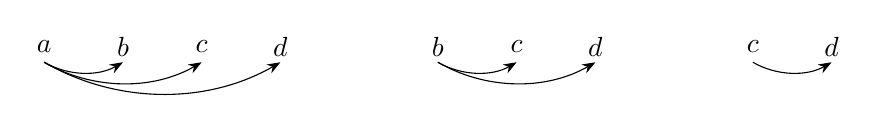
\begin{tikzpicture}[>=Stealth]
    \node at (0, 0) {$a$};
    \node at (1, 0) {$b$};
    \node at (2, 0) {$c$};
    \node at (3, 0) {$d$};
    \draw [->] (0, -0.2) arc(240:300:1);
    \draw [->] (0, -0.2) arc(240:300:2);
    \draw [->] (0, -0.2) arc(240:300:3);


    \node at (5, 0) {$b$};
    \node at (6, 0) {$c$};
    \node at (7, 0) {$d$};
    \draw [->] (5, -0.2) arc(240:300:1);
    \draw [->] (5, -0.2) arc(240:300:2);

    \node at (9, 0) {$c$};
    \node at (10, 0) {$d$};
    \draw [->] (9, -0.2) arc(240:300:1);
\end{tikzpicture}


../pic/ds3-ch2-2-7.tex

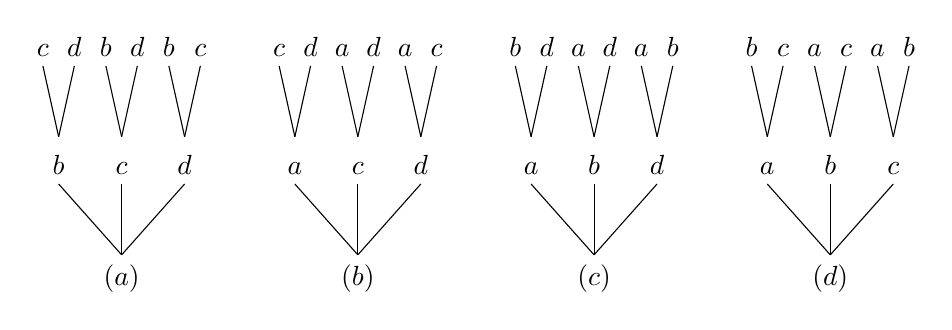
\begin{tikzpicture}[>=Stealth]
    \ExplSyntaxOn
    \tikzset{
       pics/letters/.style~n~args={3}{
            code = {
                \node at (0, 0) {$(#1)$};

                \draw (0, 0.3) -- (-0.8, 1.2) node[above] {$\clist_item:nn{#2}{1}$};
                \draw (0, 0.3) -- (0, 1.2) node[above] {$\clist_item:nn{#2}{2}$};
                \draw (0, 0.3) -- (0.8, 1.2) node[above] {$\clist_item:nn{#2}{3}$};

                \draw (-0.8, 1.8) -- (-1.0, 2.7) node[above] {$\clist_item:nn{#3}{1}$};
                \draw (-0.8, 1.8) -- (-0.6, 2.7) node[above] {$\clist_item:nn{#3}{2}$};

                \draw (0, 1.8) -- (-0.2, 2.7) node[above] {$\clist_item:nn{#3}{3}$};
                \draw (0, 1.8) -- (0.2, 2.7) node[above] {$\clist_item:nn{#3}{4}$};

                \draw (0.8, 1.8) -- (0.6, 2.7) node[above] {$\clist_item:nn{#3}{5}$};
                \draw (0.8, 1.8) -- (1.0, 2.7) node[above] {$\clist_item:nn{#3}{6}$};
            }}}
    \ExplSyntaxOff

    \draw (0,0) pic {letters={a}{b,c,d}{c,d,b,d,b,c}};
    \draw (3,0) pic {letters={b}{a,c,d}{c,d,a,d,a,c}};
    \draw (6,0) pic {letters={c}{a,b,d}{b,d,a,d,a,b}};
    \draw (9,0) pic {letters={d}{a,b,c}{b,c,a,c,a,b}};
\end{tikzpicture}


../pic/ds3-ch2-2-letters.tex

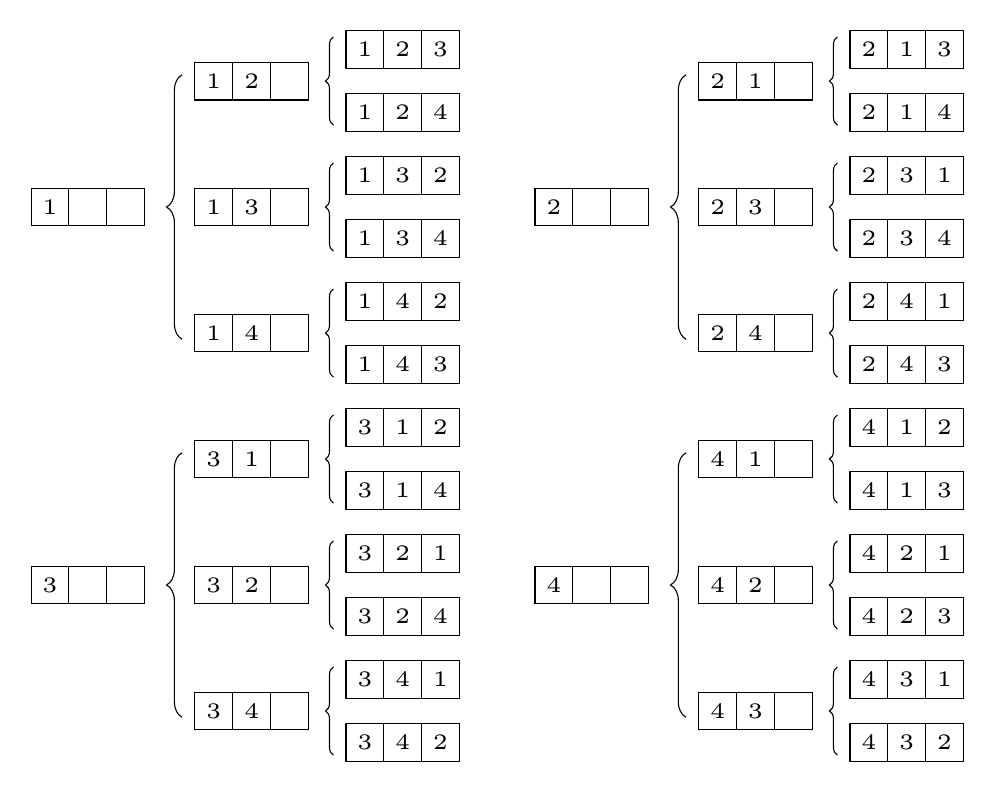
\begin{tikzpicture}[>=Stealth,
    every text node part/.style={font=\tiny},
    transform shape,
    scale=1.6]
    \tikzset{
        pics/boxes/.style n args={2}{
            code = {
                \draw (0, 0) rectangle (0.9, 0.3);
                \draw (0.3, 0) -- (0.3, 0.3);
                \draw (0.6, 0) -- (0.6, 0.3);
                \def\first{\the\numexpr(#1)/100\relax}
                \draw (0.15, 0.15) node{\first};
                \ifnum #2>1
                    \draw (0.45, 0.15) node{\the\numexpr(#1)/10 - \first*10\relax};
                    \ifnum #2>2
                        \draw (0.75, 0.15) node{\the\numexpr(#1) - \numexpr(#1)/10*10\relax};
                    \fi
                \fi
            }
        }
    }
    \tikzset{
        pics/numbers/.style n args={6}{
            code = {
                \draw (0, 0) pic {boxes={#1}{1}};

                \draw[decorate,decoration={brace,mirror,amplitude=0.2cm}] (1.2, 1.2) -- (1.2, -0.9);
                \draw (1.3,  1) pic {boxes={#1}{2}};
                \draw (1.3,  0) pic {boxes={#3}{2}};
                \draw (1.3, -1) pic {boxes={#5}{2}};

                \draw[decorate,decoration={brace,mirror,amplitude=0.1cm}] (2.4, 1.5) -- (2.4, 0.8);
                \draw (2.5, 1.25) pic {boxes={#1}{3}};
                \draw (2.5, 0.75) pic {boxes={#2}{3}};

                \draw[decorate,decoration={brace,mirror,amplitude=0.1cm}] (2.4, 0.5) -- (2.4, -0.2);
                \draw (2.5, 0.25) pic {boxes={#3}{3}};
                \draw (2.5, -0.25) pic {boxes={#4}{3}};

                \draw[decorate,decoration={brace,mirror,amplitude=0.1cm}] (2.4, -0.5) -- (2.4, -1.2);
                \draw (2.5, -0.75) pic {boxes={#5}{3}};
                \draw (2.5, -1.25) pic {boxes={#6}{3}};
            }
        }
    }

    \draw (0, 0) pic {numbers={123}{124}{132}{134}{142}{143}};
    \draw (4, 0) pic {numbers={213}{214}{231}{234}{241}{243}};

    \draw (0, -3) pic {numbers={312}{314}{321}{324}{341}{342}};
    \draw (4, -3) pic {numbers={412}{413}{421}{423}{431}{432}};
\end{tikzpicture}


../pic/ds3-ch2-2-numbers.tex

\begin{tikzpicture}[>=Stealth]
    \tikzset{
        pics/tickets/.style args={#1/#2/#3}{
        code = {
            \node at (0, 0.35) {#1};
            \node at (2, 0.7) {#2};
            \node at (2, 0) {#3};
            \draw (1.5, 0.7) -- (0.5, 0.35) -- (1.5, 0);

            \node at (5, 0) {#1};
            \node at (7, 0) {#3};
            \draw (5.5, 0) -- (6.5, 0);

            \node at (5, 0.7) {#1};
            \node at (7, 0.7) {#2};
            \draw (5.5, 0.7) -- (6.5, 0.7);
        }}}

    \draw (0, 0) pic[transform shape] {tickets=广州/北京/上海};
    \draw (0, 1.5) pic[transform shape] {tickets=上海/北京/广州};
    \draw (0, 3) pic[transform shape] {tickets=北京/上海/广州};
    \node at (0, 4.3) {起点站};
    \node at (2, 4.3) {终点站};
    \node at (6, 4.3) {飞机票};
\end{tikzpicture}


../pic/ds3-ch2-2-tickets.tex

\begin{tikzpicture}[>=Stealth, transform shape]
    \tikzset{
        pics/zuhe pailie/.style args={#1/#2/#3}{
            code = {
                \draw (-0.9, -0.4) rectangle (0.9, 0.4);
                \node at (0, 0) {$#1 \quad #2 \quad #3$};

                \draw[->] (1, 0) -- (2, 0);

                \draw (2.1, -0.6) rectangle (8.9, 0.6);
                \node at (3,  0.3) {$#1 \quad #2 \quad #3$};
                \node at (3, -0.3) {$#1 \quad #3 \quad #2$};
                \node at (5.5,  0.3) {$#2 \quad #1 \quad #3$};
                \node at (5.5, -0.3) {$#2 \quad #3 \quad #1$};
                \node at (8,  0.3) {$#3 \quad #1 \quad #2$};
                \node at (8, -0.3) {$#3 \quad #2 \quad #1$};
            }
        }
    }

    \node at (0, 1) {组 \quad 合};
    \node at (5.5, 1) {排 \quad 列};

    \draw (0, 0) pic {zuhe pailie=a/b/c};
    \draw (0, -1.6) pic {zuhe pailie=a/b/d};
    \draw (0, -3.2) pic {zuhe pailie=a/c/d};
    \draw (0, -4.8) pic {zuhe pailie=b/c/d};
\end{tikzpicture}


../pic/ds3-ch2-5-zuhe-pailie.tex

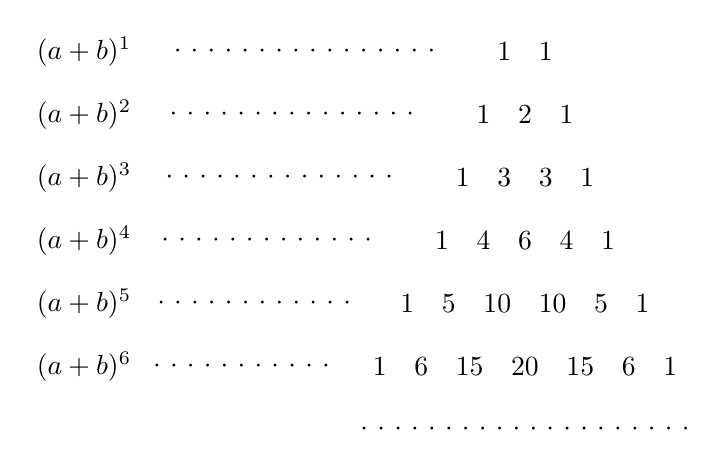
\begin{tikzpicture}[>=Stealth, scale=0.8]
    \ExplSyntaxOn
    \tikzset{
       pics/mydots/.style~n~args={1}{
            code = {
                \draw (0, 0) node {\int_step_inline:nn {#1} {$\cdot$~} } ;
            }}}
    \ExplSyntaxOff
    \draw (0, 6) node { $(a + b)^1$} (3.5, 6) pic {mydots={16}} (7, 6) node {$1 \quad 1$ };
    \draw (0, 5) node { $(a + b)^2$} (3.3, 5) pic {mydots={15}} (7, 5) node {$1 \quad 2 \quad 1$ };
    \draw (0, 4) node { $(a + b)^3$} (3.1, 4) pic {mydots={14}} (7, 4) node {$1 \quad 3 \quad 3 \quad 1$ };
    \draw (0, 3) node { $(a + b)^4$} (2.9, 3) pic {mydots={13}} (7, 3) node {$1 \quad 4 \quad 6 \quad 4 \quad 1$ };
    \draw (0, 2) node { $(a + b)^5$} (2.7, 2) pic {mydots={12}} (7, 2) node {$1 \quad 5 \quad 10 \quad 10 \quad 5 \quad 1$ };
    \draw (0, 1) node { $(a + b)^6$} (2.5, 1) pic {mydots={11}} (7, 1) node {$1 \quad 6 \quad 15 \quad 20 \quad 15 \quad 6 \quad 1$ };
   \draw (7, 0) pic {mydots={20}};
\end{tikzpicture}


../pic/ds3-ch2-7-xi-shu.tex

\begin{tikzpicture}[>=Stealth, scale=0.8]
    \NewDocumentCommand{\num}{m o} {
        \IfNoValueTF{#2}
            {\hbox {#1}}
            {\hbox{\lower-1.0ex\hbox{\scalebox{1}[0.4]{#1}}\lower.1ex\hbox{\kern-1em \scalebox{1}[0.5]{#2}}}}
    }

    \ExplSyntaxOn
    \tikzset{
       pics/line/.style~n~args={1}{
            code = {
                \int_step_inline:nnn {1}{\clist_count:n{#1}} {
                     \draw [fill=white] (##1 -1, 0) node {$\clist_item:nn{#1}{##1}$} circle (0.28);
                }
            }}}
    \ExplSyntaxOff

    \ExplSyntaxOn
    \int_step_inline:nnn {0}{5} {
        \draw (0 + 0.6*#1, 0 - #1) -- (-3.9 + 1.25 * #1, -6);
        \draw (0 - 0.65*#1, 0 - #1) -- (3.7 - 1.25 * #1, -6);
    }
    \ExplSyntaxOff

    \draw (0, 0) pic {line={\num{一}}};
    \draw (-0.65, -1) pic {line={\num{一},\num{一}}};
    \draw (-1.30, -2) pic {line={\num{一},\num{二},\num{一}}};
    \draw (-1.95, -3) pic {line={\num{一},\num{三},\num{三},\num{一}}};
    \draw (-2.60, -4) pic {line={\num{一},\num{四},\num{六},\num{四},\num{一}}};
    \draw (-3.25, -5) pic {line={\num{一},\num{五},\num{十},\num{十},\num{五},\num{一}}};
    \draw (-3.90, -6) pic {line={\num{一},\num{六},\num{十}[五],\num{二}[十],\num{十}[五],\num{六},\num{一}}};
\end{tikzpicture}


../pic/ds3-ch2-7-yang-hui-san-jiao.tex

\begin{tikzpicture}[>=Stealth, scale=0.8, transform shape]
    \tikzset{
        pics/coin/.style args={#1/#2}{
        code = {
            \draw (0, 0) node {\Large #1} circle (0.4);
            \draw (0, -0.7) node {#2};
        }}}

    \draw (0, 0) pic {coin={正/1}};
    \draw (1, 0) pic {coin={正/2}};

    \draw (3, 0) pic {coin={正/1}};
    \draw (4, 0) pic {coin={反/2}};

    \draw (0, -2) pic {coin={反/1}};
    \draw (1, -2) pic {coin={正/2}};

    \draw (3, -2) pic {coin={反/1}};
    \draw (4, -2) pic {coin={反/2}};
\end{tikzpicture}


../pic/ds3-ch3-2-coin.tex

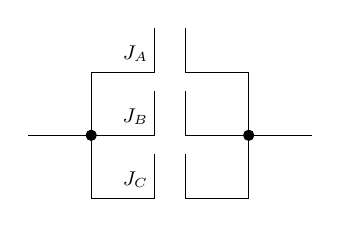
\begin{tikzpicture}[>=Stealth, scale=0.8, transform shape]
    \tikzset{
        circuit/.pic={
            \draw (0, 0) -- (2, 0) -- (2, 0.7);
            \draw (2, 1.7) -- (2, 1) -- (1, 1) -- (1, -1) -- (2, -1) -- (2, -0.3);
            \draw [fill=black] (1, 0) circle (0.08);
        }
    }
    \draw (0, 0) pic {circuit};
    \draw [xscale=-1] (-4.5, 0) pic {circuit};

    \node at (1.7, 1.3) {\small $J_A$};
    \node at (1.7, 0.3) {\small $J_B$};
    \node at (1.7, -0.7) {\small $J_C$};
\end{tikzpicture}


../pic/ds3-ch3-3-2.tex



\end{document}
